Die Kraft auf die Reckstange ist gleich gross wie die Kraft $F$, mit der die Stange den Turner hält (Wechselwirkungsprinzip). Für den Turner gilt $m\,a = F - m\,g$, also $F = m\,(g+a)$.

\begin{center}
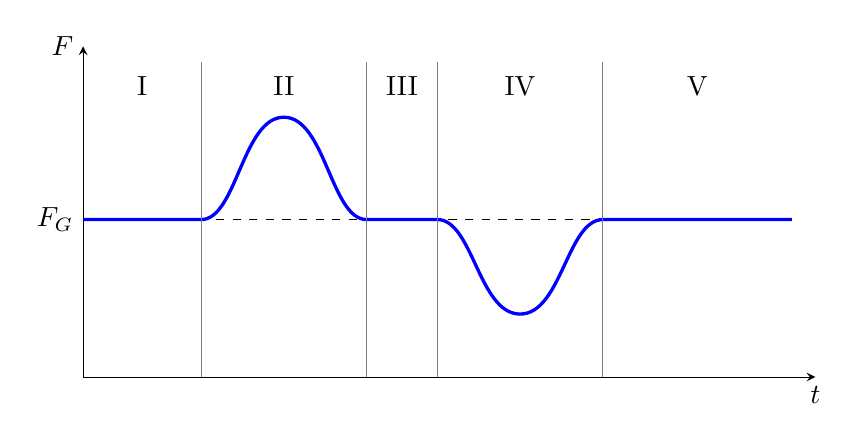
\begin{tikzpicture}[>=stealth, xscale=1.5]
 \draw[->] (0,0) -- (6.2,0) node[below] {$t$};
 \draw[->] (0,0) -- (0,4.2) node[left] {$F$};
 \draw[dashed] (0,2) -- (6,2);
 \node[left] at (0,2) {$F_\text{G}$};
 \draw[blue, very thick] (0,2) -- (1,2) .. controls (1.3,2) and (1.35,3.3) .. (1.7,3.3) .. controls (2.05,3.3) and (2.1,2) .. (2.4,2) -- (3,2) .. controls (3.3,2) and (3.35,0.8) .. (3.7,0.8) .. controls (4.05,0.8) and (4.1,2) .. (4.4,2) -- (6,2);
 \foreach \x in {1,2.4,3,4.4} \draw[gray] (\x,0) -- (\x,4);
 \node at (0.5,3.7) {I};
 \node at (1.7,3.7) {II};
 \node at (2.7,3.7) {III};
 \node at (3.7,3.7) {IV};
 \node at (5.2,3.7) {V};
\end{tikzpicture}
\end{center}

\begin{itemize}
\item[I] Streckhang in Ruhe: $F = F_\text{G}$.
\item[II] Der Turner beschleunigt nach oben ($a > 0$): $F > F_\text{G}$.
\item[III] Er bewegt sich (näherungsweise) gleichförmig nach oben: $F = F_\text{G}$.
\item[IV] Er bremst vor dem Beugehang ab ($a < 0$): $F < F_\text{G}$.
\item[V] Beugehang in Ruhe: wieder $F = F_\text{G}$.
\end{itemize}
Da der Turner am Anfang und am Ende in Ruhe ist, ist die Fläche zwischen Kurve und $F_\text{G}$-Linie in Phase II gleich gross wie in Phase IV.
